\section{Experiments}
In this section you validate your method showing the experiments that you performed. The experiments will vary depending on the project, but you might compare with previously published methods, perform an ablation study to determine the impact of various components of your system, experiment with different hyperparameters or architectural choices, use visualization techniques to gain insight into how your model works, discuss common failure modes of your model, etc. You should include graphs, tables, or other figures to illustrate your experimental results. Divide in subsections or paragraphs to help the reader navigate in your paper.

\subsection{Datasets}
\subsubsection{Own Dataset}
We gathered our own data through a web page \cite{gdpdataret} that we set up. Through it, people had the possibility to upload their own photos. As a result, we obtained a set of more than eighty folders of photos, each one belonging to a different person. On avarage, we managed to get ten photos per person.
\paragraph{Data Augmentation}
The quantity of data that we obtained is not even close to the usual amount used in large scale Deep Learning projects. So we proceeded with augmentation procedures of our training set. In particular we resorted to the Augumentor Python library \cite{augmentor}. This library allows to generate, starting from a set of images, other images, obtained from various transformations of the former set. Those transformations can be customized and can be applied randomly to each image. It follows that each augmented image is the combination of the application of a random number of transformation specified by the developer, resulting in a great variety in the augmented set.
The transformation applied, with probabilities, are:
\begin{itemize}
\item Flip left-right with probability 0.5;
\item Skew left-right with probability 1: the skew magnitude is random and varies from 0 to 0.2, which experimentally guarantees resulting images which are not deformed;
\item Alter brightness with probability 1: we perform a non linear trasformation as suggested in \cite{nonlintransf}, using parameters $\theta = 1$ and $\phi = 1$ respectively. In particular we used this transformation increasing the pixel brightness and decreasing it with probability 0.5 in both cases;
\item Adaptive equalization \cite{histeq} with probability 0.5, using a clip limit of 0.01;
\end{itemize}
In particular the last two methods were employed in order to obtain more variety of lightning conditions, which turned out to be characteristic that was lacking the most in our own dataset.
Using this augmentation procedure, we crafted five brand new images from just one, obtaining fifty images per person on our dataset.

\begin{figure}[t]
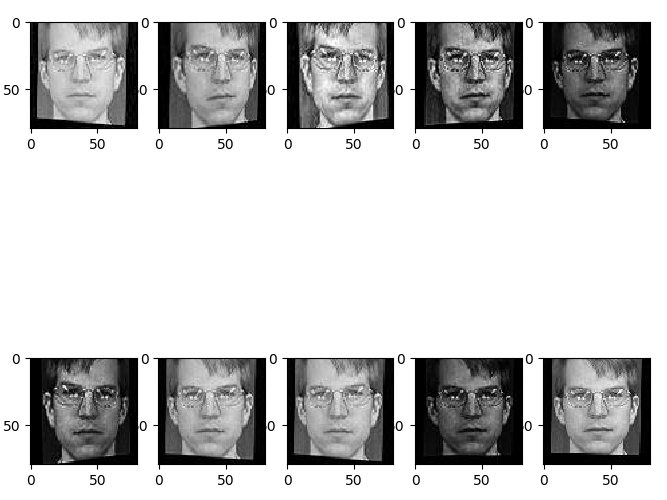
\includegraphics[width=0.8\linewidth]{images/augmented.png}
   \caption{Example of nine augmented photos obtained from a starting one, which is depicted at the bottom-right. We can see the good variety of images obtained from our augmentation procedure.}
\label{fig:long}
\label{fig:onecol}
\end{figure}

%Describe the data you are working with for your project. Usually you need to explain what type of data is it, how much data are you working with and if you applied any pre-processing, filtering, or other special treatment to use it. Remember that you have to cite each dataset you used in your project if it has been published from someone else. Instead, if you collected it by yourself you have to describe accurately how you gathered (and labeled) your data. 

\paragraph{Experiments setup.}
Here you describe all the architectural choices of your model, the hyper-parameters of your model, \eg optimizer, learning rate, momentum, batch size and if you cross-validate on them. 

\paragraph{Results and discussion.}
Discuss your results and compare with other methods. You can also perform an \emph{ablation study} on your model switching on and off some components to understand their contributions.
